% ----- Consignes exo 1 ----- %
\begin{td-exo}[Soirée chez Ramsey]\,\\ % 1 
	On considère un ensemble de six personnes. Montrer que au moins 
	trois personnes se connaissent deux-à-deux ou que au moins trois 
	personnes ne se connaissent pas deux-à-deux. 
	Est-ce vrai pour un ensemble de cinq personnes?
\end{td-exo}

% ----- Solutions exo 1 ----- %
\iftoggle{showsolutions}{
	\begin{td-sol}[]\,\\ %
		Soit \(G = (V, E)\) un graphe à six sommets. On 
		veut montrer que \(G\) contient \(K_3\) ou \(\ol{K_3}\).

		Considérons \(x\in V\) un sommet de \(G\) et procédons
		par disjonction de cas en fonction du degré de \(x\):
		\begin{itemize}
			\item Si \(\deg(x) \geq 3\), on note \(s_1, s_2, s_3\) trois voisins de \(x\).
			Si \((s_1, s_2)\in E\) alors \(x, s_1, s_2\) forment \(K_3\).
			
			De manière similaire, si \((s_1, s_3)\in E\) ou \((s_2, s_3)\in E\) alors \(K_3\) est formé.
			Si il n'existe pas d'arête entre \(s_1, s_2, s_3\) alors \(\ol{K_3}\) est formé.
			
			Ainsi, si \(\deg(x) \geq 3\) alors \(G\) contient \(K_3\) ou \(\ol{K_3}\).

			\vspace{0.1cm}
			% Figure 1
\ffigbox[\FBwidth]{
\label{Fig:td2ex9}
}{
    \fbox{
        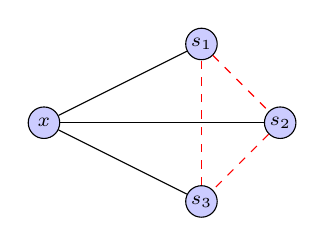
\begin{tikzpicture}[scale=1, every node/.style={circle, draw, fill=blue!20, inner sep=1pt, font=\scriptsize, minimum size=4mm}]
            \node (x) at (0, 1) {\(x\)};

            \node (s1) at (2, 2) {\(s_1\)};
            \node (s2) at (3, 1) {\(s_2\)};
            \node (s3) at (2, 0) {\(s_3\)};

            \draw (x) -- (s1);
            \draw (x) -- (s2);
            \draw (x) -- (s3);

            \draw[red, dashed] (s1) -- (s2);
            \draw[red, dashed] (s2) -- (s3);
            \draw[red, dashed] (s3) -- (s1);
        \end{tikzpicture}
    }
}

			Visuellement, on peut voir que si un des traits rouges est présent
			(donc si il existe une arête entre deux des sommets \(s_1, s_2, s_3\))
			alors \(K_3\) est formé. Sinon, il y a un triangle rouge en pointillés
			et \(\ol{K_3}\) est formé.

			\item Si \(\deg(x) \leq 2\), on note \(s_1, s_2, s_3\in V\)
			trois sommets de \(G\) qui ne sont pas voisins de \(x\) (ils
			existent forcément car \(|V| = 6\)).
			Si \((s_1, s_2)\notin E\) alors \(x, s_1, s_2\) forment \(\ol{K_3}\).

			De manière similaire, si \((s_1, s_3)\notin E\) ou \((s_2, s_3)\notin E\) alors \(\ol{K_3}\) est formé.
			Si il existe une arête entre chacun des sommets \(s_1, s_2, s_3\) alors \(K_3\) est formé.

			\vspace{0.1cm}
			% Figure 1
\ffigbox[\FBwidth]{%
\label{Fig:td1ex1c2}
}{
    \fbox{
        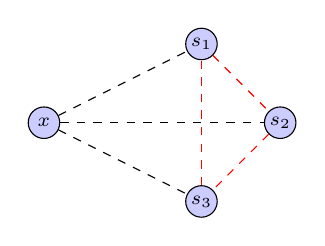
\begin{tikzpicture}[scale=1, every node/.style={circle, draw, fill=blue!20, inner sep=1pt, font=\scriptsize, minimum size=4mm}]
            \node (x) at (0, 1) {\(x\)};

            \node (s1) at (2, 2) {\(s_1\)};
            \node (s2) at (3, 1) {\(s_2\)};
            \node (s3) at (2, 0) {\(s_3\)};

            \draw[dashed] (x) -- (s1);
            \draw[dashed] (x) -- (s2);
            \draw[dashed] (x) -- (s3);

            \draw[red, dashed] (s1) -- (s2);
            \draw[red, dashed] (s2) -- (s3);
            \draw[red, dashed] (s3) -- (s1);
        \end{tikzpicture}
    }
}

			Visuellement, on peut voir que si un des traits rouges est absent
			(donc si il n'existe pas d'arête entre deux des sommets \(s_1, s_2, s_3\))
			alors \(\ol{K_3}\) est formé. Sinon, il y a un triangle rouge en pointillés
			et \(K_3\) est formé.

			Ainsi, si \(\deg(x) \leq 2\) alors \(G\) contient \(K_3\) ou \(\ol{K_3}\).
		\end{itemize}
		Donc pour un ensemble de six personnes, au moins trois personnes se connaissent deux-à-deux ou au moins trois personnes ne se connaissent pas deux-à-deux.

		Pour un ensemble de cinq personnes, le graphe \(G\) à cinq sommets
		ci-dessous ne contient ni \(K_3\) ni \(\ol{K_3}\):
		\begin{center}
			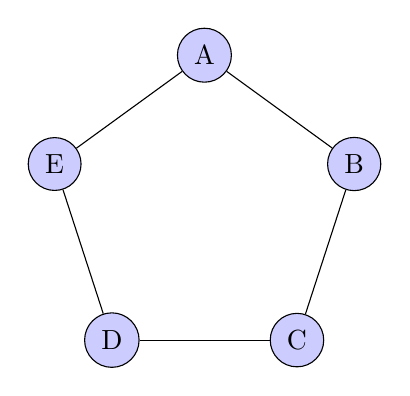
\begin{tikzpicture}[scale=1, every node/.style={circle, draw, fill=blue!20}]
				\node (A) at (90:2) {A};
				\node (B) at (18:2) {B};
				\node (C) at (-54:2) {C};
				\node (D) at (-126:2) {D};
				\node (E) at (162:2) {E};
				\foreach \from/\to in {A/B, B/C, C/D, D/E, E/A}
					\draw (\from) -- (\to);
			\end{tikzpicture}
		\end{center}
	\end{td-sol}
}{}


% ----- Consignes exo 2 ----- %
\begin{td-exo}[Hyperparcours]\,\\ % 2 
	Soit \(d\) un entier positif non nul. L'hypercube
	\(Q_d\) est le graphe dont l'ensemble des sommets est l'ensemble
	des \(d\)-uplets \(x_1,\ldots,x_d\) de 0 et de 1, deux 
	\(d\)-uplets étant adjacents s'ils diffèrent sur une seule entrée.
	\begin{enumerate}
		\item Dessiner \(Q_d\) pour \(d=1,2,3,4\).
		\item Calculer un parcours en largeur de \(Q_3\) de racine \(000\).
		En cas de choix entre plusieurs sommets pour entrer dans la file, on choisira celui
		de valeur (en binaire) minimale.
		\item Effectuer de même un parcours en profondeur de \(Q_3\).
		Cette fois, il n'y a pas de consigne en cas de choix, mais
		on essayera d'obtenir un arbre de parcours qui ne soit pas un chemin.
	\end{enumerate}
\end{td-exo}

% ----- Solutions exo 2 ----- %
\iftoggle{showsolutions}{
	\begin{td-sol}[]\, %
		\begin{enumerate}
			\item On a les hypercubes suivants:
			
			\begin{figure}[H]
	\CenterFloatBoxes{}		% centers the floatrow contents horizontally
	\begin{floatrow}
		% Figure 1
\ffigbox[\FBwidth]{
\caption{\centering \,\\Hypercube \(Q_1\)}\label{Fig:qd1}
}{
    \fbox{
        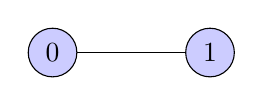
\begin{tikzpicture}[scale=1, every node/.style={circle, draw, fill=blue!20}]
            \node (A) at (0, 0) {0};
            \node (B) at (2, 0) {1};
            \foreach \from/\to in {A/B} \draw (\from) -- (\to);
        \end{tikzpicture}
    }
}

		% Figure 2
\ffigbox[\FBwidth]{
\caption{\centering \,\\Hypercube \(Q_2\)}\label{Fig:qd2}
}{
    \fbox{
        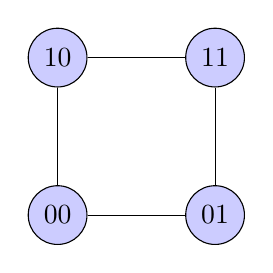
\begin{tikzpicture}[scale=1, every node/.style={circle, draw, fill=blue!20}]
            \node (A) at (0, 0) {00};
            \node (B) at (2, 0) {01};
            \node (C) at (2, 2) {11};
            \node (D) at (0, 2) {10};
            \foreach \from/\to in {A/B, B/C, C/D, D/A} \draw (\from) -- (\to);
        \end{tikzpicture}
    }
}

		% Figure 3
\ffigbox[\FBwidth]{
\caption{\centering \,\\Hypercube \(Q_3\)}\label{Fig:qd3}
}{
    \fbox{
        % Q3: Cube (Hypercube of dimension 3)
        \begin{tikzpicture}[scale=1, every node/.style={circle, draw, fill=blue!20, inner sep=1pt, font=\scriptsize}]
            % Parameters
            \def\L{2}            % side length of square
            \def\dx{0.9} \def\dy{0.6} % offset for the "back" square (gives perspective)

            % front (lower) square: coordinates ordered 000,001,011,010 (clockwise)
            \coordinate (v000) at (0,0);
            \coordinate (v001) at (\L,0);
            \coordinate (v011) at (\L,\L);
            \coordinate (v010) at (0,\L);

            % back (shifted) square: add (dx,dy) and these will be 100,101,111,110
            \coordinate (v100) at ($ (v000) + (\dx,\dy) $);
            \coordinate (v101) at ($ (v001) + (\dx,\dy) $);
            \coordinate (v111) at ($ (v011) + (\dx,\dy) $);
            \coordinate (v110) at ($ (v010) + (\dx,\dy) $);

            % draw edges front square
            \foreach \a/\b in {v000/v001, v001/v011, v011/v010, v010/v000}
                \draw (\a) -- (\b);

            % draw edges back square
            \foreach \a/\b in {v100/v101, v101/v111, v111/v110, v110/v100}
                \draw (\a) -- (\b);

            % connect corresponding vertices (cube edges)
            \foreach \a/\b in {v000/v100, v001/v101, v011/v111, v010/v110}
                \draw (\a) -- (\b);

            % nodes with labels (binary strings)
            \node at (v000) {000};
            \node at (v001) {001};
            \node at (v011) {011};
            \node at (v010) {010};
            \node at (v100) {100};
            \node at (v101) {101};
            \node at (v111) {111};
            \node at (v110) {110};
        \end{tikzpicture}
    }
}
	\end{floatrow}
\end{figure}

\begin{figure}[H]
	\CenterFloatBoxes{}		% centers the floatrow contents horizontally
	\begin{floatrow}
		% Figure 4
\ffigbox[\FBwidth]{
\caption{\centering Hypercube \(Q_4\)\\Noeuds non précisés pour la clareté}\label{Fig:qd4}
}{
    \fbox{
        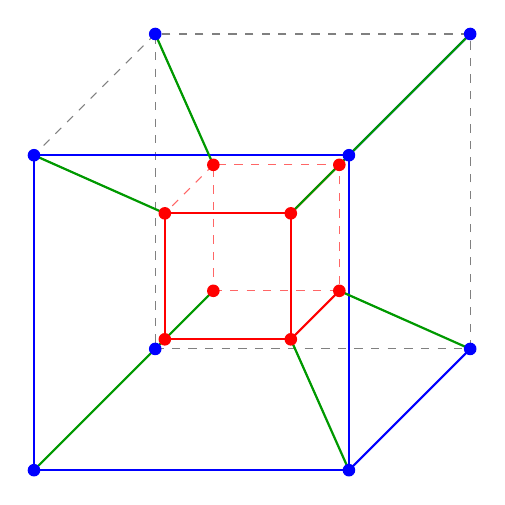
\begin{tikzpicture}[scale=2, line join=round]
            % Define the vertices of the outer cube
            \coordinate (A1) at (0,0,0);
            \coordinate (B1) at (2,0,0);
            \coordinate (C1) at (2,2,0);
            \coordinate (D1) at (0,2,0);
            \coordinate (E1) at (0,0,2);
            \coordinate (F1) at (2,0,2);
            \coordinate (G1) at (2,2,2);
            \coordinate (H1) at (0,2,2);
            
            % Define the vertices of the inner cube (offset)
            \coordinate (A2) at (0.6,0.6,0.6);
            \coordinate (B2) at (1.4,0.6,0.6);
            \coordinate (C2) at (1.4,1.4,0.6);
            \coordinate (D2) at (0.6,1.4,0.6);
            \coordinate (E2) at (0.6,0.6,1.4);
            \coordinate (F2) at (1.4,0.6,1.4);
            \coordinate (G2) at (1.4,1.4,1.4);
            \coordinate (H2) at (0.6,1.4,1.4);
            
            % Draw the outer cube (hidden edges dashed)
            \draw[dashed, gray] (A1) -- (B1) -- (C1) -- (D1) -- cycle; % bottom face
            \draw[dashed, gray] (A1) -- (E1);
            \draw[dashed, gray] (D1) -- (H1);
            \draw[blue, thick] (B1) -- (F1);
            \draw[blue, thick] (C1) -- (G1);
            \draw[blue, thick] (E1) -- (F1) -- (G1) -- (H1) -- cycle; % top face
            
            % Draw the inner cube (hidden edges dashed)
            \draw[dashed, red!60] (A2) -- (B2) -- (C2) -- (D2) -- cycle; % bottom face
            \draw[dashed, red!60] (A2) -- (E2);
            \draw[dashed, red!60] (D2) -- (H2);
            \draw[red, thick] (B2) -- (F2);
            \draw[red, thick] (C2) -- (G2);
            \draw[red, thick] (E2) -- (F2) -- (G2) -- (H2) -- cycle; % top face
            
            % Draw connecting edges between outer and inner cubes (tesseract edges)
            \draw[green!60!black, thick] (A1) -- (A2);
            \draw[green!60!black, thick] (B1) -- (B2);
            \draw[green!60!black, thick] (C1) -- (C2);
            \draw[green!60!black, thick] (D1) -- (D2);
            \draw[green!60!black, thick] (E1) -- (E2);
            \draw[green!60!black, thick] (F1) -- (F2);
            \draw[green!60!black, thick] (G1) -- (G2);
            \draw[green!60!black, thick] (H1) -- (H2);
            
            % Add small dots at vertices for clarity
            \foreach \point in {A1,B1,C1,D1,E1,F1,G1,H1}
                \fill[blue] (\point) circle (0.04);
            \foreach \point in {A2,B2,C2,D2,E2,F2,G2,H2}
                \fill[red] (\point) circle (0.04);
        \end{tikzpicture}
    }
}
	\end{floatrow}
\end{figure}

			\item On peut effectuer le parcours suivant:
			\begin{equation*}
				000 \to 001 \to 101 \to 100 \to 110 \to 010 \to 011 \to 111
			\end{equation*}
			ce qui se représente visuellement comme suit:

			% Figure 3
\ffigbox[\FBwidth]{
\caption{\centering \,\\Hypercube \(Q_3\)}\label{Fig:qd3}
}{
    \fbox{
        % Q3: Cube (Hypercube of dimension 3)
        \begin{tikzpicture}[scale=1, every node/.style={circle, draw, fill=blue!20, inner sep=1pt, font=\scriptsize}]
            % Parameters
            \def\L{2}            % side length of square
            \def\dx{0.9} 
            \def\dy{0.6}         % offset for the "back" square (gives perspective)
            \def\offset{0.15}    % offset distance from cube edges
            
            % front (lower) square: coordinates ordered 000,001,011,010 (clockwise)
            \coordinate (v000) at (0,0);
            \coordinate (v001) at (\L,0);
            \coordinate (v011) at (\L,\L);
            \coordinate (v010) at (0,\L);
            
            % back (shifted) square: add (dx,dy) and these will be 100,101,111,110
            \coordinate (v100) at ($ (v000) + (\dx,\dy) $);
            \coordinate (v101) at ($ (v001) + (\dx,\dy) $);
            \coordinate (v111) at ($ (v011) + (\dx,\dy) $);
            \coordinate (v110) at ($ (v010) + (\dx,\dy) $);
            
            % draw edges front square
            \foreach \a/\b in {v000/v001, v001/v011, v011/v010, v010/v000}
                \draw[gray!50] (\a) -- (\b);
            
            % draw edges back square
            \foreach \a/\b in {v100/v101, v101/v111, v111/v110, v110/v100}
                \draw[gray!50] (\a) -- (\b);
            
            % connect corresponding vertices (cube edges)
            \foreach \a/\b in {v000/v100, v001/v101, v011/v111, v010/v110}
                \draw[gray!50] (\a) -- (\b);
            
            % Path: 000 → 001 → 101 → 100 → 110 → 010 → 011 → 111
            
            % Arrow 1: 000 → 001 (bottom edge, offset downward)
            \draw[->, very thick, red!70!black] 
                ($ (v000) + (0.1,-\offset) $) -- ($ (v001) + (-0.1,-\offset) $);
            \node[draw=none, fill=white, inner sep=1pt, font=\tiny, text=red!70!black] 
                at ($ (v000)!0.5!(v001) + (0,-\offset-0.25) $) {1};
            
            % Arrow 2: 001 → 101 (right-back edge, offset right/down)
            \draw[->, very thick, red!70!black] 
                ($ (v001) + (\offset,0) $) -- ($ (v101) + (\offset,0) $);
            \node[draw=none, fill=white, inner sep=1pt, font=\tiny, text=red!70!black] 
                at ($ (v001)!0.3!(v101) + (\offset+0.3,0) $) {2};
            
            % Arrow 3: 101 → 100 (back edge, offset back/up)
            \draw[->, very thick, red!70!black] 
                ($ (v101) + (-0.1,\offset) $) -- ($ (v100) + (0.1,\offset) $);
            \node[draw=none, fill=white, inner sep=1pt, font=\tiny, text=red!70!black] 
                at ($ (v101)!0.52!(v100) + (0,\offset+0.2) $) {3};
            
            % Arrow 4: 100 → 110 (left-back edge, offset left/back)
            \draw[->, very thick, red!70!black] 
                ($ (v100) + (-\offset,0.1) $) -- ($ (v110) + (-\offset,-0.1) $);
            \node[draw=none, fill=white, inner sep=1pt, font=\tiny, text=red!70!black] 
                at ($ (v100)!0.5!(v110) + (-\offset-0.2,0) $) {4};
            
            % Arrow 5: 110 → 010 (left front-back edge, offset left)
            \draw[->, very thick, red!70!black] 
                ($ (v110) + (-\offset,0) $) -- ($ (v010) + (-\offset,0) $);
            \node[draw=none, fill=white, inner sep=1pt, font=\tiny, text=red!70!black] 
                at ($ (v110)!0.4!(v010) + (-\offset-0.25,0.1) $) {5};
            
            % Arrow 6: 010 → 011 (left-top edge, offset upward)
            \draw[->, very thick, red!70!black] 
                ($ (v010) + (0.1,\offset) $) -- ($ (v011) + (-0.1,\offset) $);
            \node[draw=none, fill=white, inner sep=1pt, font=\tiny, text=red!70!black] 
                at ($ (v010)!0.6!(v011) + (0,-\offset-0.1) $) {6};
            
            % Arrow 7: 011 → 111 (right front-back edge, offset right)
            \draw[->, very thick, red!70!black] 
                ($ (v011) + (\offset,0) $) -- ($ (v111) + (\offset,0) $);
            \node[draw=none, fill=white, inner sep=1pt, font=\tiny, text=red!70!black] 
                at ($ (v011)!0.3!(v111) + (\offset+0.3,0) $) {7};
            
            % nodes with labels (binary strings) - drawn last to be on top
            \node at (v000) {000};
            \node at (v001) {001};
            \node at (v011) {011};
            \node at (v010) {010};
            \node at (v100) {100};
            \node at (v101) {101};
            \node at (v111) {111};
            \node at (v110) {110};
        \end{tikzpicture}
    }
}
		\end{enumerate}
	\end{td-sol}
}{}


% ----- Consignes exo 3 ----- %
\begin{td-exo}[Convexité]\,\\ % 3 
	% fill
\end{td-exo}

% ----- Solutions exo 3 ----- %
\iftoggle{showsolutions}{
	\begin{td-sol}[]\,\\ %
		A remplir %TODO solve exercise 3
	\end{td-sol}
}{}


% ----- Consignes exo 4 ----- %
\begin{td-exo}[Convexité]\,\\ % 4 
	% fill
\end{td-exo}

% ----- Solutions exo 4 ----- %
\iftoggle{showsolutions}{
	\begin{td-sol}[]\,\\ %
		A remplir %TODO solve exercise 4
	\end{td-sol}
}{}


% ----- Consignes exo 5 ----- %
\begin{td-exo}[Convexité]\,\\ % 5 
	% fill
\end{td-exo}

% ----- Solutions exo 5 ----- %
\iftoggle{showsolutions}{
	\begin{td-sol}[]\,\\ %
		A remplir %TODO solve exercise 5
	\end{td-sol}
}{}


% ----- Consignes exo 6 ----- %
\begin{td-exo}[Convexité]\,\\ % 6 
	% fill
\end{td-exo}

% ----- Solutions exo 6 ----- %
\iftoggle{showsolutions}{
	\begin{td-sol}[]\,\\ %
		A remplir %TODO solve exercise 6
	\end{td-sol}
}{}


% ----- Consignes exo 7 ----- %
\begin{td-exo}[Convexité]\,\\ % 7 
	% fill
\end{td-exo}

% ----- Solutions exo 7 ----- %
\iftoggle{showsolutions}{
	\begin{td-sol}[]\,\\ %
		A remplir %TODO solve exercise 7
	\end{td-sol}
}{}


% ----- Consignes exo 8 ----- %
\begin{td-exo}[Convexité]\,\\ % 8 
	% fill
\end{td-exo}

% ----- Solutions exo 8 ----- %
\iftoggle{showsolutions}{
	\begin{td-sol}[]\,\\ %
		A remplir %TODO solve exercise 8
	\end{td-sol}
}{}


% ----- Consignes exo 9 ----- %
\begin{td-exo}[Convexité]\,\\ % 9 
	% fill
\end{td-exo}

% ----- Solutions exo 9 ----- %
\iftoggle{showsolutions}{
	\begin{td-sol}[]\,\\ %
		A remplir %TODO solve exercise 9
	\end{td-sol}
}{}


% ----- Consignes exo 10 ----- %
\begin{td-exo}[Convexité]\,\\ % 10 
	% fill
\end{td-exo}

% ----- Solutions exo 10 ----- %
\iftoggle{showsolutions}{
	\begin{td-sol}[]\,\\ %
		A remplir %TODO solve exercise 10
	\end{td-sol}
}{}


% ----- Consignes exo 11 ----- %
\begin{td-exo}[Convexité]\,\\ % 11 
	% fill
\end{td-exo}

% ----- Solutions exo 11 ----- %
\iftoggle{showsolutions}{
	\begin{td-sol}[]\,\\ %
		A remplir %TODO solve exercise 11
	\end{td-sol}
}{}